%!TEX root = ../dissertation.tex
\begin{savequote}[75mm]
We must be prepared to accept the possibility that what we call ``the environment'' may lie, in part, within the skin of the biological organism
\qauthor{Herbert Simon (\citeyear{simon1955behavioral})}
\end{savequote}

% \chapter{Formalism}
\Chapter[Meta-level Markov decision processes]{Formalism}
% \begin{flushright}
% {\large\itshape Meta-level Markov decision processes}
% \vspace{1.3\baselineskip}
% \end{flushright}

\newthought{The key insight} behind the proposed framework is that cognitive processes are solutions to sequential decision problems. Drawing on a subfield of artificial intelligence known as \emph{rational metareasoning} \citep{matheson1968economic,russell1991principles}, we formalize this insight using the framework of \emph{metalevel Markov decision processes} (metalevel MDPs; \citealp{hay2012selecting}). In this framework, a cognitive process is formalized as a sequential process of executing computational actions that update an agent's mental state. At each moment, the agent must choose whether to continue thinking, refining their mental state but accruing computational cost, or to instead stop thinking and take action. In the former case, they must additionally decide which computation to execute next (i.e., what to think about). In the latter case, they select the action that seems best given their current mental state and receive a reward associated with the external utility of that action.

% in the latter case, they select the optimal action given their current belief and receive a reward associated with the external utility of that action.

\todo{Define object-level?}

In this chapter, I provide a formal description of the framework. The formalization presented here is an adaptation from the framework as proposed in \citet{hay2016principles}. We have modified the framework somewhat to better facilitate the specification of cognitive models.

% We begin by introducing Markov decision processes (MDPs). Next, we define metalevel MDPs as extensions of standard MDPs. Finally, we define a specific metalevel MDP model for multi-attribute decision-making, which we will employ in our experimental case studies.

% Below, we give a high-level and intuitive overview of the general framework and its application to multi-attribute choice, the domain we will use in our case studies. A formal treatment is provided in Appendix~\ref{metamdp}.

% We begin by describing, in intuitive terms, how the framework can be applied to model multi-attribute decision-making. Next, we will formally define metalevel MDPs. Finally, we will return to the multi-attribute decision-making case, showing how the formalism can be applied to a specific case.

\begin{figure*}
  % \centering
  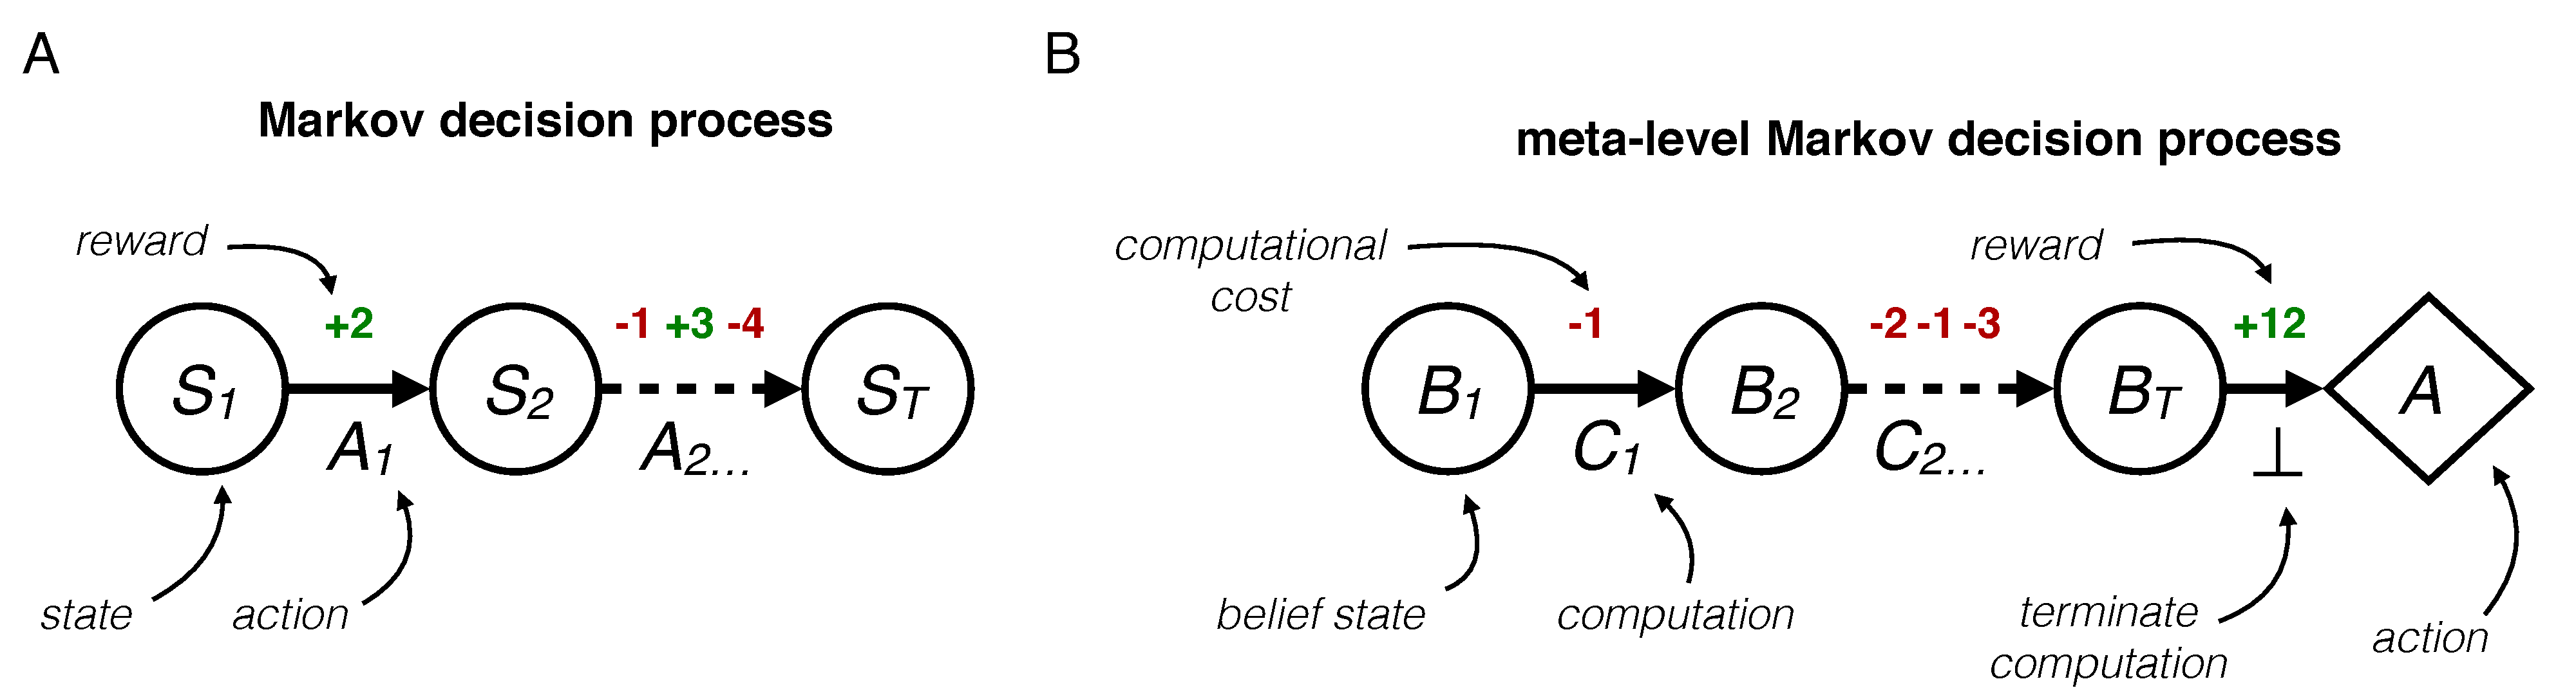
\includegraphics[width=\textwidth]{figs/metamdp.pdf}
  \caption{\captiontitle{Meta-level Markov decision processes.}
  \subcap{A} A Markov decision process formalizes the problem of acting adaptively in a dynamic environment. The agent executes actions that change the state of the world and generate rewards, which the agent seeks to maximize.
  \subcap{B} A \emph{metalevel} Markov decision process formalizes the problem of \emph{deciding how to act} when computational resources are limited. The agent executes computations that update their belief state and incur computational cost. When the agent executes the termination operation $\bot$, they take an external action based on their current belief state.}
  \label{fig:metamdp-diagram}
\end{figure*}


\section{Markov decision processes}

A metalevel Markov decision process is an extension of a standard Markov decision process (MDP) illustrated in \Fig{fig:metamdp-diagram}{a}. Thus, we begin with a brief overview of standard MDPs. See \citet{sutton2018reinforcement} for a more thorough overview.

MDPs are the standard formalism for modeling the sequential interaction between an agent and a stochastic environment. An MDP is defined by a set of states $\S$, a set of actions $\A$, a transition function $T$, and a reward function $R$. A state $s \in \S$ specifies the relevant state of the world. An action $a \in \A$ is an action the agent can perform. The transition function $T: \S \times \A \rightarrow \Delta(\S)$\footnotemark{} encodes the dynamics of the world as a distribution of possible future states for each possible previous state and action. Finally, the reward function $R: \S \times \A \rightarrow \R $ specifies the reward or utility for executing a given action in a given state. We additionally assume an initial state $s_0$ which the environment is initialized in and a set of terminal state $\S_\bot$ such that the episode ends when the agent reaches one of those states.

\footnotetext{%
  $\Delta(\S)$ denotes the set of all distributions over the set $\S$. Note that this definition is equivalent to the more standard style of defining the transition function as a probability mass function (i.e., $T: \S \times \A \times \S \rightarrow [0, 1])$. However, defining transition functions in this way is often highly unintuitive. We will thus instead define transition functions as generative probabilistic models. This notation reflects that choice.
}


\subsection{Optimal policies and value functions}

The solution to an MDP is a policy $\pi: \S \rightarrow \Delta(\A)$ that (stochastically) selects which action to perform next given the current state. That is, $a_t \sim \pi(s_t)$. The goal is to find a policy that maximizes the expected cumulative reward attained, that is, the \emph{return}. The optimal policy is thus defined,
\begin{equation}\label{eq:optimal-policy}
  \pi^* = \argmax_\pi \expect{
    \sum_{t=1}^{t_\bot} R(s_t, a_t)
  }{
   a_t \sim \pi(s_t)
  },
\end{equation}
where $t_\bot$ is the timepoint at which the episode terminates (when $s_{t+1} \in \S_\bot$). Note that the expectation implicitly conditions on the transition function, i.e., $s_{t+1} \sim T(s_t, a_t)$.

How can we identify such a policy? This question is the subject of a huge field of research in articifical intelligence, and countless methods have been developed. Many of these methods draw on the concept of a \emph{value function}. The \emph{state} value function (or just ``value function'') is defined
%
\begin{equation}\label{eq:state-value}
  V^\pi(s) = \expect{
    \sum_{t=1}^{t_\bot} R(s_t, a_t)
  }{
   s_1 = s,\ a_t \sim \pi(s_t)
  }.
\end{equation}
%
It specifies the expected total reward one will receive if one begins in state $s$ and selects actions according to the policy $\pi$. Similarly, the \emph{action} value function (or ``state-action value function'') is defined
%
\begin{equation}\label{eq:action-value}
  Q^\pi(s, a) = \expect{
    \sum_{t=1}^{t_\bot} R(s_t, a_t)
  }{
   s_1 = s,\ a_1 = a,\ a_{t \neq 1} \sim \pi(s_t)
  }.
\end{equation}
%
The action value function just like the state value function except that it also specifies the first action to be taken. 

The value functions for the optimal policy are called the optimal value functions. They can be defined simply $V^* = V^{\pi^*}$ and $Q^* = Q^{\pi^*}$. By combining Equations~\ref{eq:optimal-policy}, \ref{eq:state-value}, and~\ref{eq:action-value}, we can see that the optimal value functions specify the maximal expected reward one could expect to gain begining with a given state (and action) under any policy.

Putting aside for now the problem of identifying the these functions (see \citealp{puterman2014markov}), the optimal policy\footnote{%
  To be more precise, the equation below defines the \emph{maximum entropy} optimal policy, that is, the optimal policy whose action distributions are maximally random. For simplicity, we will refer to the maximum entropy optimal policy as simply ``the'' optimal policy.
} can be defined as simply
%
\begin{equation}\label{eq:argmaxQ}
  \pi^*(s) = \text{Uniform}\left(\argmax_a Q^*(s, a)\right).
\end{equation}
%
That is, the optimal policy selects the action that produces the greatest expected long-term reward, breaking ties randomly. When modeling human data, one typically assumes that this maximization is performed imperfectly. In particular, we will assume that actions are drawn according to a softmax (or Boltzmann distribution),
%
\begin{equation}
  \pi(a \mid s) \propto \expp{\beta \cdot Q^*(s, a)}
\end{equation}
% \displaystyle\sum_{a'} \expp{\beta \cdot Q^*(s, a')}
%
where the inverse-temperature parameter $\beta$ controls how well the policy maximizes, behaving completely randomly when $\beta = 0$ and approaching the optimal policy as $\beta \rightarrow \infty$.

This concludes our brief overview of MDPs. We are now ready to describe metalevel MDPs.

% An important property of MDPs is that there is at least one deterministic \emph{optimal policy}; that is, there is a mapping from states to actions that, when followed, will produce the maximum possible return. 

\section{Meta-level Markov decision processes}

% The concept is thus very similar to \emph{elementary information processes} \citep{chase1978elementary,simon1979information,posner1982information,payne1988adaptive}. 

Meta-level Markov decision processes (metalevel MDPs) extend the standard MDP formalism to model the sequential decision problem posed by resource-bounded computation \citep{hay2012selecting}. Like a standard MDP, a metalevel MDP is defined by sets of states and actions, and transition and reward functions. However, the states corresponded to beliefs (mental states) and the actions correspond to computations (cognitive operations). The metalevel transition function describes how computations update beliefs, and the metalevel reward function captures the costs (e.g., time) and benefits (e.g., better decisions) of computation.

Formally, we define a metalevel MDP by a set of beliefs $\M$, a set of computations $\C$, a transition function $T$, and a reward function $R$. These four components are analagous to the states, actions, transition function, and reward function in a standard MDP. We additionally define a set of world states $\W$, upon which the transition and reward functions depend. This is the only formal distinction between a metalevel MDP and a standard MDP. However, as we discuss in Section~\ref{sec:metamdp-marginalized}, we can convert metalevel MDPs into equivalent MDPs by marginalizing over the world state.\footnote{This is similar to the \emph{belief MDP} transformation of a partially observable MDP (POMDP). see Section~\ref{sec:metamdp-pomdp} for additional discussion on the relation between metalevel MDPs and POMDPs.}


% In the remainder of this chapter, we will describe the components of metalevel MDPs in greater detail, provide a simple example metalevel MDP, and discuss strategies for finding good metalevel policies.

\subsection{Two models of computation}

Before we further describe the components of metalevel MDPs, it is useful to first establish the basic conceptual model of computation on which they rely. As pointed out by \citet[Chapter~7]{hay2016principles}, there are at least two such models, each with its own advantages.

In the \emph{mechanical} model, computations are viewed as internal actions that update the agent's internal state. These can be contrasted with external actions that update the state of the environment---but they are fundamentally the same type of thing. This view is highlighted in Figure~\ref{fig:sequential-intuition}. It should be familiar to cognitive scientists, as it is the view underlying most process-level psychological models, including, for example, evidence accumulation models and cognitive architectures \todo{reference intro?}.

In the \emph{Bayesian} model, computations are viewed as experiments that generate information about the world \citep{matheson1968economic}. The results of these experiments are synthesized, by Bayesian inference, into estimates of the utility of different possible external actions, thus informing the agent's choice of which action to take. While the notion of Bayesian inference will not be new for most cognitive scientists, this view is quite different from the standard Bayesian approach in cognitive science (e.g., \citealp{tenenbaum2011how}). In particular, while the standard approach treats cognition as a problem of drawing inferences given data, this view treats cognition as a problem of generating the data that drives inference. In this way, the Bayesian model of computation resembles cognitive models of active learning \citep{gureckis2012selfdirected,gottlieb2013informationseeking}.\footnote{We further discuss links between metalevel MDPs and active learning in the \todo{conclusion}}

Importantly, the two models are not mutually exclusive. They are often compatible interpretations of a single system. The mechanical model emphasizes the process of computation, while the Bayesian model emphasizes its function. In this way, the mechanical and Bayesian models are analagous to Marr's algorithmic and computational levels. Unlike in Marr's levels, however, adopting the Bayesian model is more than just an interpretation; it has practical consequences for what one can do with the model. Specifically, it puts constraints on the types of computation one can consider. All Bayesian models have a mechanical interpretation, but not vice versa. On the other hand, adopting the Bayesian interpretation makes it much easier to identify optimal policies for metalevel MDPs. Specifically, it allows us to convert a metalevel MDP into a standard MDP, which is a critical step for the model-based solution strategies we employ. We discuss this transformation, including the constraints it imposes on the metalevel MDP, in Section~\ref{sec:metamdp-marginalized}.

All metalevel MDPs in this dissertation have both mechanical and Bayesian interpretations, but which interpretation is foregrounded will vary. In Chapter~\ref{sec:attention}, we will strongly emphasize the Bayesian interpretation, modeling eye fixations as sampling information to update beliefs about utility of the available options. In Chapters~\ref{sec:memory} and~\ref{sec:planning}, we will emphasize the mechanical interpretation, modeling the fluctuating accessibility of memories and the construction of decision trees. However, in all cases, both interpretations are useful---not just practically, but also as conceptual tools to better understand the cognitive process.

\separator

We are now ready to formally specify the components of a metalevel MDP. A metalevel MDP is defined by a tuple $(\W, \M, \C, T, R)$ specifying the set of world states, the set of mental states, the set of computations, and the transition and reward functions. We describe each of these components in turn.


\subsection{World states}
A world state $w \in \W$ captures the state of the world that is relevant to the agent's current task. For example, in a decision-making task, the world state might define the utility of the various actions available to the agent (as in Chapter~\ref{sec:attention}). In a memory task, the world state might correspond to the strength of the memory that the agent is trying to recall (Chapter~\ref{sec:memory}). More formally, the world state includes any information that is not known to the agent, but affects either the reward or transition functions.

\subsection{Mental states}

% \todo{maybe instead of m(w), use p_m(w)}
A mental state $m \in \M$ captures the agent's internal state, as relevant to the task at hand. The interpretation of a mental state can vary, in particular based on whether one is adopting the mechanical or Bayesian view. 

When adopting the Bayesian view, mental states correspond to \emph{beliefs}, formally, posterior distribution over the world state. For example, in Chapter~\ref{sec:attention}, a mental state will correspond to a posterior distribution over the utilities of the items in a choice set. Mapping mental states to Bayesian beliefs is powerful because it provides a formal link between mental states and world states. We will use the notation $b_m$ to denote the Bayesian belief associated with mental state $m$. For example, we denote the probability of a world state given a mental state as $b_m(w) = \Pr(W = w \mid M = m)$.\footnote{%
  For notational convenience, we assume in this chapter that $\W$ is countable.
} Simlarly, we denote expectations about functions of the world state given the mental state as $\expectunder{f(w)}{w \sim b_m}$. When it is clear from context, we will drop the subscript, e.g., using $b_t$ in place of $b_{m_t}$. 

When adopting the mechanical view, mental states can take on a broader set of interpretations. In many cases, mental states are naturally interpreted as a \emph{representation} of the task at hand. This interpretation is quite natural in Chapter~\ref{sec:planning}, where mental states correspond to partially constructed decision trees (see also \citealp[Chapter 5]{hay2016principles}). Here, the mental state is a representation of a set of possible solutions to the object-level problem (that is, a set of plans). However, a mental state may also capture features of the agent's internal state that are not naturally conceptualized as representations. For example, in Chapter~\ref{sec:memory}, the mental state specifies the activation level of a memory (see also \citealp{suchow2016deciding}).

As mentioned above, it is often useful to adopt \emph{both} the Bayesian and mechanical views. In particular, having a Bayesian interpretation makes it possible to convert the metalevel MDP into an equivalent MDP. However, when primarily adopting the mechanical view (i.e., not directly specifying the mental states as beliefs), some care must be taken to ensure that the transformation is possible. Specifically, the mental state must be a \emph{sufficient statistic} for the full history of mental states and computations, with respect to the world state (c.f. \citealp{kaelbling1998planning}; see Section~\ref{sec:metamdp-sufficient} for details).

In addition to specifying the set of possible mental states $\M$, one must additionally specify an initial mental state, $m_0$. When adopting the Bayesian interpretation, $m_0$ corresponds to a prior distribution over the world state, $b_0$. By default, we will assume that this prior is accurate, i.e., $b_0(w) = \Pr(W=w)$. However, in Chapter~\ref{sec:attention}, we will need to assume some bias in the initial mental state to fully capture human behavior.

% One typically makes distributional assumptions that restrict the space of beliefs the agent can entertain, such that $\M \subset \Delta(\S)$. 

% Importantly, however, contrary to a standard rational treatment of beliefs, the belief states in a metalevel MDP do not include all the information that is available to the agent. Instead, the belief state only contains information that is immediately accessible, excluding, for example, long-term memories and the number of calories in every box of cereal on a shelf.

\subsection{Computations}
A computational operation $c \in \C$ is a primitive operation afforded by the agent's cognitive architecture. Formally, it is a metalevel action that updates the mental state in much the same way as an object-level action changes world state. In a metalevel MDP model, all cognition can be broken down into a sequence of these computations, but the model makes no attempt to explain how those basic operations are themselves implemented. The concept is thus very similar to \emph{elementary information processes} \citep{chase1978elementary,simon1979information,posner1982information,payne1988adaptive}. 

All metalevel MDPs include a special computation, the termination operation denoted by $\bot$, which indicates that computation should be terminated. In a decision-making context, this results in an external action being selected, specifically, the one that has maximal expected utility given the current mental state. In other contexts (e.g. memory recall in Chapter~\ref{sec:memory}), it may correspond to giving up on a cognitively demanding task. In either case, the most fundamental metalevel problem---how long to compute---is captured by the decision about when to execute $\bot$.

\subsection{Transition function}
The transition function $T: \M \times \C \times \W \rightarrow \Delta(\M)$ describes how computation updates mental states. Formally, $T(m, c, w)$ is a distribution of possible new mental states that would result from performing a computation $c$ in mental state $m$ when the true state of the world is $w$. At each time step, the next mental state is sampled from this distribution:
\begin{equation}
m_{t+1} \sim T(m_t, c_t, w).
\end{equation}

When fully adopting the Bayesian view, computations correspond to experiments that generate information about the world state, which is integrated into a belief by Bayesian inference. The transition function describes this process. Formally, each computation defines a state-dependent distribution of observations $p_c(o \mid w)$. Given the previous mental state $m_t$ (and associated belief $b_t$) and the observation $o_t$, the new mental state $m_{t+1}$ is defined such that
%
\begin{equation}\label{eq:bayes-update}
  b_{m_{t+1}}(w) = p(w | m_t, o_t) = \frac{
    p_c(o_t \mid w) b_{m_t}(w) 
  }{
    p(o_t \mid m_t, c_t)
    % \displaystyle\sum_{w' \in \W} b_{m_t}(w') p_c(o_t \mid w')
  },
\end{equation}
%
where the second equality is the application of Bayes rule, updating the prior $b_{m_t}$ given the likelihood $p_c(o \mid w)$. The transition function describes the full process of sampling an observation and updating the belief accordingly. Denoting the update in Equation~\ref{eq:bayes-update} as ``bayes-update'', the full transition function is defined
%
\begin{align}
  o_t &\sim p_c(\cdot \mid w) \\
  m_{t+1} &= \text{bayes-update}(m_t, o_t, p_c)
\end{align}

When adopting the mechanical view, the transition function can have arbitrary form. However, in order to convert the metalevel MDP into an equivalent MDP, one must define the transition function such that the mental state remains a sufficient statistic (Section~\ref{sec:metamdp-sufficient}).

Regardless of which view is adopted, terminating computation (executing $\bot$) always transitions to a terminal state, $m_\bot$. That is,
%
\begin{equation}
  T(m_t, \bot, w) = \text{Uniform}(\{m_\bot\})
\end{equation}
%


% This formalization is quite natural for many types of cognitive operations, such as memory recall and mental simulation. However, it can also be applied in less obvious cases; for example, performing an addition operation generates previously inaccessible information about the value of the sum of two numbers.

% the marginalized metalevel transition function is always stochastic. Without knowledge of the true object-level state $s$, the agent cannot predict exactly how a computation will change her belief---if she could, she could simply adopt that updated belief without performing the computation. 

\subsection{Reward function}
The metalevel reward function $R: \M \times \C \times \W \rightarrow \R$ describes both the costs and benefits of computation. For the former, $R$ assigns a strictly negative reward for all non-terminating computational operations,
%
\begin{equation}
R(m, c, w) = -\cost(m, c) \text{ for } c \neq \bot.
\end{equation}
%
We assume that the cost of a computation can depend on the current mental state (e.g., to model switching costs in Chapter~\ref{sec:attention}) but not on the state of the world. The cost of computation may include multiple factors. At a minimum, it captures the opportunity cost of the time spent executing the computation (rather than taking actions in the world). The simplest choice is to assume a constant cost for each computation executed.

Intuitively, the benefit of computation is that it yields more useful mental states, those that allow us to behave more effectively in the world. The benefit of computation is thus captured by the reward for the termination operation $\bot$,
%
\begin{equation}
  R(m, \bot, w) = \utility(m, w),
\end{equation}
%
where $\utility(m, w)$ describes how ``good'' the belief is, given the true state of the world. What ``good'' means depends on the type of cognitive process one is modeling. 

In a decision-making context (Chapters~\ref{sec:attention} and~\ref{sec:planning}), terminating computation corresponds to selecting an object-level action $a \in \A$ to execute in the world. A good mental state is one that leads one to choose a good action. Formally, the reward for termination is defined as the true utility of the external action that the agent would execute given the current belief. Letting $U(w, a)$ denote the object-level utility of executing action $a$ in the world state $w$, we have
%
\begin{equation}\label{eq:term-reward}
\utility(m, w) = U\left(w, \pi\act(m)\right).
\end{equation}
%
where $\pi\act: \M \rightarrow \Delta(\A)$ is an \emph{action selection policy} that chooses an action to take based on the current mental state. When adopting the Bayesian view, we will define
\begin{equation}
  \pi\act(m) = \text{Uniform} \left(\argmax_a \expectunder{U(w, a)}{w \sim b_m}\right).
\end{equation}
%
That is, the action selection policy randomly selects one of the actions that has maximal expected utility given the current mental state. When adopting the mechanical view, we will assume that the mental state contains sufficient information to quickly choose an action (i.e., without much additional computation). For example, in Chapter~\ref{sec:planning}, the mental state is a decision tree, a data structure that keeps track of the best plan identified so far.

Note that this type of termination reward can be also applied to sequential object-level problems by defining $\A$ as a set of abstact actions (or \emph{options}; \citealp{sutton1999mdps}) that correspond to sequences of concrete actions. This does require that all computation is executed before any object-level action is performed, but this constraint does not reduce performance when the object-level transition function is deterministic. See Chapter~\ref{sec:planning} for an application to deterministic sequential problems and \todo{conclusion} for a discussion of the problem of interleaved computation and action.

Outside of decision-making contexts, the benefits of computation can take a broader form. For example, if one simply seeks to form accurate beliefs, the utility of a mental state could be the probability assigned to the true world state: $\utility(m, w) = b_m(w)$. Another general class defines a set of mental states as goal states $\M_{\mathrm{goal}} \subset \M$, with a positive reward associated with reaching\footnote{We assume that the policy always terminates in a goal state, as any reasonable policy would do.} a goal state,
%
\begin{equation}\label{eq:goal-term}
  \utility(m, w) = \begin{cases}
    1 &\text{if } m \in \mathcal{M}_{\mathrm{goal}} \\
    0 &\text{otherwise}
  \end{cases}
\end{equation}
%
For example, in Chapter~\ref{sec:memory}, we will associate a positive reward with reaching a mental state where the activation of a memory exceeds a threshold associated with recall.


\section{Metalevel policies}\label{sec:metamdp-policy}

If a metalevel MDP defines the problem a cognitive process must solve, a metalevel policy defines the solution. It is a strategy for selecting which cognitive operation to execute next given the current mental state. Formally, the policy, $\pi: \M \rightarrow \Delta(\C)$, is a mapping from beliefs to distributions over computations. At each time step, the next computation is drawn from this distribution, $c_t \sim \pi(m_t)$.

How should we determine this policy? The classical cognitive modeling approach is to specify a plausible strategy, perhaps motivated by aspects of human behavior. In Chapter~\ref{sec:planning}, we show how classical heuristics for decision-tree search can be naturally modeled as policies in a metalevel MDP. However, in the resource-rational approach pursued here, we take a different approach. Specifically, we are interested in the \emph{optimal policy} for the metalevel MDP. Paralleling Equation~\ref{eq:optimal-policy}, the optimal metalevel policy is defined
%
\begin{equation}\label{eq:optimal-meta-policy}
  \pi^* = \argmax_\pi \expect{
    \sum_{t=1}^{t_\bot} R(m_t, c_t, w)
  }{
    c_t \sim \pi(m_t)
  }.
\end{equation}
That is, it maximizes the expected return. In a metalevel MDP the return can be broken down into two components capturing the costs and benefits of computation,
\begin{equation}
  \pi^* = \argmax_\pi \expect{
    \utility(m_{t_\bot}, w) - \sum_{t=1}^{t_\bot-1} \cost(m_t, c_t)
  }{
    c_t \sim \pi(m_t)
  }.
\end{equation}
This emphasizes that the optimal policy is the cognitive strategy that best trades off between the costs and benefits of computation. 

Unfortunately, identifying optimal metalevel policies is substantially more challenging than writing down their definition. In Section~\ref{sec:computing}, we discuss various strategies for tackling this problem. But first, we will discuss how metalevel MDPs can be converted to standard MDPs, an important step in many solution strategies.

% In addition to being a solution to a metalevel MDP, we can also think of a policy as a cognitive model, one which makes predictions about the sequence of cognitive operations a person will perform when performing some task. If we make assumptions about how those cognitive operations generate process-tracing data, for example eye fixations (Chapter~\ref{sec:attention}) or mouse clicks (Chapter~\ref{sec:planning}), the policy (along with the transition function) corresponds to a likelihood model over those data. 


\section{Marginalized metalevel MDPs}\label{sec:metamdp-marginalized}

Although metalevel MDPs have the same basic structure as an MDP, they are distinct in that the transition and reward functions depend on a world state, $w$, that is unknown to the agent. One unfortunate consequence of this difference is that many of the standard tools for finding optimal policies of MDPs cannot be directly applied. Fortunately, when certain requirements are met, one can convert a metalevel MDP into a standard MDP by marginalizing the world state out of the transition and reward functions.

In the following sections we define the marginal transition and reward functions, providing analytic expressions when possible. We then specify the sufficient-statistic constraint necessary for the transformation to be correct.

\subsection{Marginal transition function}
The marginal transition function $T: \M \times \C \rightarrow \Delta(\M)$ can be defined easily in generative form:
%
\begin{equation}
\begin{aligned}
  w &\sim b_{m_t}\\
  m_{t+1} &\sim T(m_t, c_t, w).
\end{aligned}
\end{equation}
%
One simply samples the world state from the belief before applying the transition dynamics. This is sufficient to sample from $T(m, c)$. However, we will often need an explicit proabability mass function, which is defined
%
\begin{equation}
T(m_{t+1} \mid m_t, c_t) = \expectunder{T(m_{t+1} \mid m_t, c_t, w)}{w \sim b_{m_t}}.
\end{equation}
This expression cannot be simplified in the general case. In practice, we will work with Gaussian or discrete beliefs that make this integration tractable.

\subsection{Marginal reward function}
The marginal reward function $R: \M \times \C \rightarrow \R$ is defined
%
\begin{equation}
R(m, c) = \expectunder{R(m, c, w)}{w \sim b_m}.
\end{equation}
%
For $c \neq \bot$, $R(m, c, w)$ does not depend on $w$, and we have simply
%
\begin{equation}
  R(m, c) = -\text{cost}(m, c).
\end{equation}
The reward for terminating, however, may depend on the state of the world; we must marginalize it out:
%
\begin{equation}\label{eq:marginal-term}
  R(m, \bot) = \expectunder{\utility(m, w)}{w \sim b_m}.
\end{equation}
%
In the decision-making context (Equation~\ref{eq:term-reward}), this marginalization is straightforward. The utility of a belief is simply the maximal expected utility of any action given that belief:
%
\begin{equation}
\begin{aligned}
R(m, \bot)
&= \expectunder{\utility(m, w)}{w \sim b_m} \\
&= \expectunder{U(w, \pi\act(m))}{w \sim b_m} \\
&= \expectunder{U\left(w,\, \argmax_a \expectunder{U(w', a)}{w' \sim b_m}\right)}{w \sim b_m} \\
&= \max_a \expectunder{U(w, a)}{w \sim b_m}
.
\end{aligned}
\end{equation}
The final line follows from
%
\begin{math}
  f\left(\argmax_a f(a)\right) = \max_a f(a)
  ,
\end{math}
%
where $f(a)$ is $\expectunder{U(w, a)}{w \sim b_m}$.\footnote{%
  For clarity, we here assume a single optimal action. It is easy to see that 
}

Outside of a decision-making context, we will only consider goal-based belief utility functions (Equation~\ref{eq:goal-term}), which do not depend on the world state. In the general case, one would have to derive a model-specific expression for Equation~\ref{eq:marginal-term}, just as one must do for the transition function.

\subsection{Sufficient statistic requirement}\label{sec:metamdp-sufficient}

As briefly mentioned above, marginalizing a metalevel MDP is only possible when the mental state is a sufficient statistic for the full history of mental states and computations with respect to the world state. Formally, we must have that
%
\begin{equation}\label{eq:sufficient}
  p(w \mid m_t) = p(w \mid \vec{m}_{1:t}, \vec{c}_{1:t}).
\end{equation}
%

To see why this is, note that a key property of a Markov decision process is the Markov property. That is, the probability of the next state depends only on the current state and action; formally,
\begin{equation}\label{eq:markov}
  p(m_{t+1} \mid m_t, c_t) = p(m_t \mid \vec{m}_{1:t}, \vec{c}_{1:t}).
\end{equation}
where $\vec{m}_{1:t}$ is the complete history of mental states. Making explicit the marginalization over $w$ on each side of the equation, we have
\begin{equation}
  \sum_w p(w | m_t, c_t) p(m_{t+1} | m_t, c_t, w) =
  \sum_w p(w | \vec{m}_{1:t}, \vec{c}_{1:t}) p(m_{t+1} | m_t, c_t, w).
\end{equation}
From this it is clear that 
%
\begin{equation}
  p(w | m_t, c_t) = p(w | \vec{m}_{1:t}, \vec{c}_{1:t})
\end{equation}
%
Finally, noting that $p(w | m_t, c_t) = p(w | m_t)$, we arrive at Equation~\ref{eq:sufficient}. Thus, the Markov property (Equation~\ref{eq:markov}) implies the sufficiency of the mental state (Equation~\ref{eq:sufficient}), meaning that we cannot have the Markov property without ensuring that the mental state is a sufficient statistic. This in turn means that the marginalized metalevel MDP can only be a \emph{Markov} decision process if the mental state is a sufficient statistic.

\section{Relation to partially observable Markov decision processes}

Partially observable Markov decision process (POMDPs; \citealp{kaelbling1998planningb}) are generalizations of MDPs where the agent does not know the state, but instead receives an observation conditional on the state and action at each time step: $o_t \sim O(s_{t+1}, a_t)$. Given these observations, the agent maintains a belief about the current state using a Bayesian update similar to Equation~\ref{eq:bayes-update} but additionally accounting for the possibility that the state changes,
%
\begin{equation}\label{eq:pomdp-update}
  b_{t+1}(s_{t+1}) = p(s_{t+1} | b_t, o_t) = \frac{
    O(o_t \mid s_{t+1}, a_t) \displaystyle\sum_{s_t \in \S} T(s_{t+1} \mid s_t, a_t) b_t(s_t)
  }{
    p(o_t \mid b_t, a_t)
  } 
\end{equation}
%

Metalevel MDPs that fully adopt the Bayesian intepretation of beliefs can be understood as a constrained form of a POMDP in which the state never changes. In this case, the belief update reduces to
\begin{equation}\label{eq:pomdp-update}
  b_{t+1}(s) =  
  \frac{O(o_t \mid s, a_t) b_t(s)}{p(o_t \mid b_t, a_t)}
\end{equation}
which is exactly analagous to Equation~\ref{eq:bayes-update}.
 % but with $w$ replaced by $s$ and $p_c(o_t \mid w)$ by $O(o_t \mid s, a_t)$
Metalevel MDPs additionally require that all but one action yield strictly negative reward and that the remaining action, $\bot$, leads to a terminal state.

When adopting the mechanical view, however, this interpretation is less natural (when it is possible at all). This is particularly problematic outside of decisoin making contexts. For example, in Chapter~\ref{sec:memory}, the mental state will capture the activation level of a memory. 

, this formulation is not as natural. In this case, one can think of the state as being composed of two elements, $b$ and $w$, the former being observable and the latter not.


\section{Identifying good metalevel policies}\label{sec:computing}

Here we discuss a few general methods for identifying optimal (or at least reasonable) policies for metalevel MDPs. Following Equation~\ref{eq:argmaxQ}, the optimal metalevel policy can be expressed as
%
\begin{equation}
  \pi^*(m) = \text{Uniform}\left(\argmax_b Q^*(m, c)\right).
\end{equation}


\subsection{Dynamic programming}\label{sec:backinduct}

For metalevels MDPs with sufficiently small state spaces, the most robust and accurate method for identifying an optimal policy is dynamic programming. See \citet{sutton2018reinforcement} and \citet{puterman2014markov} for a general overview of these methods. Here, we provide a brief introduction and a few practical suggestions for applying this approach to metalevel MDPs.

\todo{decide what to do with this section}

When the belief space is finite and discrete, dynamic programming can be applied directly. Sometimes, the belief space will be infinite in principle, but can be made finite by placing an upper bound on the number of computations that can be performed.





However, almost always, the belief space naturally decomposes along the time step. That is, there is 

Formally, the belief space can be broken down into disjoint subsets, one for each time point,
% %
% \begin{equation}
%   \M = \bigcup_t^T \M_t.
% \end{equation}
% %
% In this case, backwards induction is generally the most efficient strategy.\footnote{
%   Backwards induction performs each possible Bellman backup exactly once (one for each pair of beliefs that have non-zero transition probability), wheres other algorithms like value iteration generally perform each backup many times.
% } In this strategy, one begins by computing the value of each possible belief at the maximum time step, $T$. By definition, this value is
% %
% \begin{equation}
%   V(b_T) = R(m, \bot)  %\ \forall\  b_T \in \M_t
% \end{equation}
% %
% Then one computes the value of executing each possible computation beliefs at the previous time step, $T-1$, as
% %
% \begin{equation}
%   Q(b_{T-1}, c) = \sum_{b_T} T(b_T \mid b_{T-1}, c) V(b_T) - \cost(b_{T-1}, c)
% \end{equation}
% %

but structured, one can take advantage of symmetry in the space to reduce its effective size, sometimes dramatically so. One way to accomplish this is to use a cache-based dynamic programming scheme with a key function that collapses across states that are functionally equivalent. For example, in Chapter~\ref{sec:planning}, we use a key function that processes a decision tree recursively, using a commutative operation (summation) to combine the keys for subtrees whose roots are siblings.

When the belief space is continuous and low-dimensional, we discretize the space into evenly spaced bins, being careful to set the range such that the optimal policy almost never reaches the end points. We then specify a maximum number of computations (ideally one imposed by the task itself, e.g., a time limit), and use backwards induction to compute the value function. In many cases, computing the marginalized transition function is the computational bottleneck. Thus, when possible, we precompute any aspects of this calculation that will be needed multiple times. For example, in Chapter~\ref{sec:memory}, we precompute the transition function for single item and reuse this precomputed table to determine transition probabilities when there are two items.


If the belief space is continuous and high-dimensional, or discrete and without symmetry structure, dynamic programming is not likely to be tracatable. In this case, an approximate method is required. We disucss a few approximations in the following sections.

\subsection{The myopic policy}

In their pioneering work on metareasoning \citet{russell1991principles} suggested an approximation to rational metareasoning by one-step look-ahead, what they called the metalevel greedy approximation. This policy, which we call the myopic policy (following \citealp{hay2012selecting}), is defined
\begin{equation}
  \pi\myopic(m) = \text{Uniform}\left(\argmax_b Q\myopic(m, c)\right),
\end{equation}
where
\begin{equation}
Q\myopic(m, c) = \E_{m' \sim T(\cdot \mid m, c)}\left[ 
  R(m', \bot)
\right] - \cost(m, c)
\end{equation}
with $Q\myopic(m, \bot) = R(m', \bot)$. The myopic action value function, $Q\myopic$ gives the expected termination reward after performing one more computation, less the cost of that computation. Thus, the myopic policy selects each computation as if it will be the last one executed.

\subsection{Multi-step lookahead}

The problem with the myopic policy is that it systematically underestimates the value of computation. This leads it to stop computing too early. To take a simple example, consider a metalevel MDP in which each computation generates one piece of binary evidence in favor of one action vs. another. If the current belief has two pieces of evidence in favor of action A ($m = +2$),\footnote{Note that for this metalevel MDP to have a Bayesian interpretation, the belief state must also include the number of computations performed.} then there is no way that a single computation will change the decision the agent will make. The next belief will be either $+1$ or $+2$, and A will be the action with maximal expected value in either case. Clearly there is no benefit to executing a single computation, so the myopic policy will terminate. However, given the opportunity to execute multiple computations, the tide could easily be swayed in favor of action B. If computation is not very costly, it would likely be worth computing more.

\citet{gabaix2005bounded} proposed a solution to this problem for information-gathering problems similar to metalevel MDPs. In the so-called \emph{directed cognition} model, the policy selects from sequences of computations, similar to options in hierarchical reinforcement learning \citep{sutton1999mdps}. Thus, if a any sequence of computations has a better expected value than terminating, the policy will continue to compute. Note that when applying this strategy, one need not actually commit to taking the full sequence of computations that previously had maximal value, as the outcome of the first comuptation may make another computation (or sequence of computations) more valuable.

\citet{hay2012selecting} proposed another solution to this problem, based on the idea that a solution to a complex metalevel MDP can approximated by composing solutions to a set of simplified metalevel MDPs, specifically MDPs taht formalize the problem of deciding how to decide between one object-level action and the expected return of its best alternative.

one possible solution to this problem, the \emph{blinkered approximation}. The intuition behind this approximation is approximate the solution to a complex metalevel MDP 


Each of these smaller metalevel MDPs includes only the computations for reasoning about the expected return of the corresponding object-level action.
While this \textit{blinkered} approximation is more accurate than the meta-greedy policy, it is also significantly less scalable and not directly applicable to metareasoning about planning.



This policy selects computations by making a myopic approximation to the VOC:
\begin{equation}
\pi\myopic(m) = \text{Uniform}\left(\argmax_c \VOC\myopic(m, c)\right).
\end{equation}
where
\begin{equation*}
  \VOC\myopic(m,c) = \E_{m' \sim T(m, c)}\left[
    R(m',\bot)
  \right] - \cost(m,c) - R(m, \bot)
\end{equation*}
and $\VOC\myopic(m,\bot)$ is defined to be 0. $\VOC\myopic$ specifies the amount of reward one would gain by executing one more computation before terminating, rather than terminating immediately. When working with the VOC, 



To build additional intuition, we can break down the VOC into two terms, capturing the value of information produced by computation and the cost of computation, respectively:
%
\begin{equation}
  Q^*(m_t, c_t) = 
    \underbrace{R(m_t, \bot)
    }_{
      \substack{\text{current}\\ \text{decision}\\ \text{quality}}
    } +
    \underbrace{
      \underbrace{
        \E[R(b_T, \bot)] - R(m_t, \bot)
      }_{
        \text{value of information}
      } - 
      \underbrace{
        \E\left[\sum_{i=t}^T \cost(b_i, c_i) \right]
      }_{
        \text{cost of computation}
      }
    }_{
      \text{value of computation}
    }.
\end{equation}
%



Historically, rational metareasoning \citep{russell1991principles} has been defined in terms of a slightly different quantity, the \emph{value of computation} (VOC). 

\subsection{The value of computation}
The VOC is exactly what it sounds like; it specifies the value of performing a computation, where ``value'' refers to the long-term value in the same sense as the action value function, $Q^*$. Indeed, VOC can be defined in terms of $Q^*$: $\VOC(m, c) = Q^*(m, c) - R(m, \bot)$. Intuitively, the VOC is the amount of reward one can gain by executing a computation (and then continuing to select computations optimally) rather than making a choice immediately. It is easy to see that maximizing VOC is equivalent to maximizing $Q^*$, and so we can equivalently define the optimal metalevel policy as
%
\begin{equation}
  \pi^*(m) = \text{Uniform}\left(\argmax_b \VOC(m, c)\right).
\end{equation}
%
Thus, VOC and $Q^*$ contain essentially the same information. In practice, we will use $Q^*$ when solving metalevel MDPs with dynamic programming, and VOC when approximating solutions using ideas from rational metareasoning.

To build additional intuition, we can break down the VOC into two terms, capturing the value of information produced by computation and the cost of computation, respectively:
%
\begin{equation}
  Q^*(m_t, c_t) = 
    \underbrace{R(m_t, \bot)
    }_{
      \substack{\text{current}\\ \text{decision}\\ \text{quality}}
    } +
    \underbrace{
      \underbrace{
        \E[R(b_T, \bot)] - R(m_t, \bot)
      }_{
        \text{value of information}
      } - 
      \underbrace{
        \E\left[\sum_{i=t}^T \cost(b_i, c_i) \right]
      }_{
        \text{cost of computation}
      }
    }_{
      \text{value of computation}
    }.
\end{equation}
%




Thus, the policy executes the computation that will provide the greatest expected improvement in the termination reward at the next step less the cost of that computation; if this value is not positive for any computation, it terminates.

The myopic policy can be quite effective in some cases. However, it terminates computation too early because it systematically underestimates


% \begin{equation}
%     % \text{VOC}_1(c,m_t)=\mathds{E}\left[r\meta(B_{t+1},\bot) | m_t,c_t \right] +r\meta(m_t,c) - r\meta(m_t,\bot),
%     \text{VOC}_1(c,m) = \expectunder{r\meta(B', \bot)} - r\meta(m,\bot) + r\meta(m,c),
%     % \text{VOC}_1(c,m) = \expect[B'\sim T\meta(m,c,\cdot)]{U(B')} - U(m) + r\meta(m,c),
  
% \end{equation}
% %
%
is the myopic value of computation \cite{Russell1991}. The meta-greedy policy selects each computation assuming that it will be the last computation. 
This policy is optimal when computation provides diminishing returns (i.e. the improvement from each additional computation is less than that from the previous one), but it deliberates too little when this assumption is violated.
For example, in the tornado problem (where false negatives have high cost), a single simulation may be unable to ensure that evacuation is unnecessary with sufficient confidence, while two or more could.
% For instance, when the outcome of simulating an action is binary, either outcome of a single simulation may be insufficient to change the agent's decision---rendering the myopic VOC negative---whereas two or more simulations might change it and thus have a positive VOC when the stakes are high.

Hay et al. (2012) approximated rational metareasoning by combining the solutions to smaller metalevel MDPs that formalize the problem of deciding how to decide between one object-level action and the expected return of its best alternative.
Each of these smaller metalevel MDPs includes only the computations for reasoning about the expected return of the corresponding object-level action.
While this \textit{blinkered} approximation is more accurate than the meta-greedy policy, it is also significantly less scalable and not directly applicable to metareasoning about planning. %when applied to sequential decision problems where the value of each object-level action depends on which actions will be taken afterwards.
%\footnote{Hay et al. present an application of their method to MCTS in Go, but they only use their method at the root node, effectively reducing the problem to a bandit problem.}

%It has been proposed that people approximate optimally selecting individual computations by metareasoning over a small subset of all possible sequences of computations \cite{Milli2017}. The solution to this simplified problem can be approximated efficiently \cite{LiederGriffiths2017}, but this approximation neglects the sequential nature of selecting individual computations.
These are the main approximations to rational metareasoning. So, to date, there appears to be no accurate and scalable method for solving general metalevel MDPs.


This suggests a strategy for selecting computations optimally. For each item, estimate how much one's decision would improve if one sampled from it (and then continued sampling optimally). Subtract from this number the cost of taking the sample (and also the estimated cost of the future samples). Now identify the item for which this value is maximal. If it is positive, it is optimal to take another sample for this item; otherwise, it is optimal to stop sampling and make a decision.

This basic logic is formalized in rational metareasoning as the \textit{value of computation} (VOC; \citealp{russell1991principles}). Formally, $\VOC(m, c)$ is defined as the expected increase in total metalevel reward if one executes a single computation, $c$, and continues optimally rather than making a choice immediately (i.e., executing $\bot$):
$$
\VOC(m_t, c) = R(m_t, c) + \E \left[
  \sum_{t'=t+1}^T R(b_{t'}, c_{t'})\ \Big\vert\ c_{t'} \sim \pi^*(b_{t'}) 
\right] - R(m, \bot).
$$

We can then define the optimal policy as selecting computations with maximal VOC:
$$
\pi^*(m) \sim \text{Uniform}(\argmax{c} \VOC(m, c)).
$$
For those familiar with reinforcement learning, this recursive joint definition of $\pi^*$ and VOC is exactly analogous to the joint definition of the optimal policy with the action value function, $Q$ \citep{sutton2018reinforcement}. Indeed, $\VOC(m, c) = Q(m, c) - R(m, \bot)$. 

\subsection{Optimal metalevel policy}

\todo{shorten, maybe move some material to metamdp section}

The solution to a metalevel MDP takes the form of a Markov policy, $\pi$, that stochastically selects which computation to take next given the current belief state. Formally, $c_t \sim \pi(m_t)$. The optimal metalevel policy, $\pi^*$, is the one that maximizes expected total metalevel reward,
\begin{equation*}
  \pi^* = \argmax{\pi} \E \left[ \sum_t^T R(m_t, c_t) \ \Big\vert\ c_t \sim \pi(m_t) \right].
\end{equation*}
Replacing $R$ with its definition, we see that this requires striking a balance between the expected value of the chosen item and the computational cost of the samples that informed the choice,
\begin{equation*}
  \pi^* = \argmax{\pi} \E \left[
     \max_i \mu_T^{(i)} - \sum_t^{T-1} \cost(m_t, c_t)
   \ \Big\vert\ c_t \sim \pi(m_t) \right].
\end{equation*}
That is, one wishes to acquire accurate beliefs that support selecting a high-value item, while at the same time minimizing the cost of the samples necessary to attain those beliefs. This suggests a strategy for selecting computations optimally. For each item, estimate how much one's decision would improve if one sampled from it (and then continued sampling optimally). Subtract from this number the cost of taking the sample (and also the estimated cost of the future samples). Now identify the item for which this value is maximal. If it is positive, it is optimal to take another sample for this item; otherwise, it is optimal to stop sampling and make a decision.

This basic logic is formalized in rational metareasoning as the \textit{value of computation} (VOC; \citealp{russell1991principles}). Formally, $\VOC(m, c)$ is defined as the expected increase in total metalevel reward if one executes a single computation, $c$, and continues optimally rather than making a choice immediately (i.e., executing $\bot$):
$$
\VOC(m_t, c) = R(m_t, c) + \E \left[
  \sum_{t'=t+1}^T R(b_{t'}, c_{t'})\ \Big\vert\ c_{t'} \sim \pi^*(b_{t'}) 
\right] - R(m, \bot).
$$
In our model, this can be rewritten
$$
\VOC(m_t, c) = -\cost(m_t, c) + \E \left[ 
  \max_i \mu_T^{(i)} - \sum_{t'=t+1}^{T-1} \cost(b_{t'}, c_{t'})
  \Big\vert\ c_{t'} \sim \pi^*(b_{t'})
\right] -  \max_i \mu_t^{(i)}.
$$
That is, the VOC for sampling a given item in some belief state is the expected improvement in the value of the chosen item (rather than making a choice based on the current belief) minus the cost of sampling that item and the expected cost of all future samples.

We can then define the optimal policy as selecting computations with maximal VOC:
$$
\pi^*(m) \sim \text{Uniform}(\argmax{c} \VOC(m, c)).
$$
For those familiar with reinforcement learning, this recursive joint definition of $\pi^*$ and VOC is exactly analogous to the joint definition of the optimal policy with the action value function, $Q$ \citep{sutton2018reinforcement}. Indeed, $\VOC(m, c) = Q(m, c) - R(m, \bot)$. 

Finally, by definition, $\VOC(m,\bot)=0$ for all $m$. Thus, the optimal policy terminates sampling when no computation has a positive VOC.

\subsection{Bayesian metalevel policy search}\label{sec:BMPS}

This method is based on an approximation of the VOC as a linear combination of features,
\begin{equation}\label{eq:vochat}
  \begin{aligned}
    \VOCapprox =& w_{1}\VOImy(m,c)+w_{2}\VPIitem(m,c) +
     w_{3}\VPI(m) -(\cost(c)+w_{4}),
  \end{aligned}
\end{equation}
for all $c\neq\bot$, with $\widehat{\VOC}(m, \bot; \vec{w}) = \VOC(m,\bot)=0$.

We briefly define the features here, and provide full derivations in Appendix~\ref{app:attention-derivations}. The VOI terms quantify the \textit{value of information} \citep{howard1966information} that might be gained by different additional computations. Note that the VOI is different from the VOC because the latter includes the costs of computation as well as its benefits. In general, the VOI is defined as the expected improvement in the utility of the action selected based on additional information rather than the current belief state: $E_{\tilde{m} \mid m}[R(\tilde{m}, \bot) - R(m, \bot)]$, where $\tilde{m}$ is a hypothetical future belief in which the information has been gained, the distribution of which depends on the current belief.

$\VOImy(m,c)$ denotes the expected improvement in choice utility from drawing one additional sample from item $c$ before making a choice, as opposed to making a choice immediately based on the current belief, $m$. $\VPIitem(m,c)$ denotes the expected improvement from learning the true value of item $c$, and then choosing the best item based on that information. Finally, $\VPI(m)$ denotes the improvement from learning the true value of \text{every} item and then making an optimal choice based on that complete information.

Together, these three features approximate the expected value of information that could be gained by the (unknown) sequence of future samples. Importantly, this true value of information always lies between the lower bound of $\VOImy$ and the upper bound of $\VPI$ (see \Fig{fig:attention-voi}), implying that the true VOI is a convex combination of these two terms. Note, however, that the weights on this combination are not constant across beliefs, as assumed in our approximation. Thus, including the $\VPIitem$ term, improves the accuracy of the approximation, by providing an intermediate value between the two extremes. Finally, the last two terms in Equation~\ref{eq:vochat} approximate the cost of computation: $\cost(c)$ is the cost of carrying out computation $c$ and $w_{4}$ approximates the expected future costs incurred under the optimal policy.

Although maximizing $\VOCapprox$ identifies the policy with the best performance, it is unlikely that humans make attentional decisions using such perfect and noiseless maximization. Thus, 
we assume that computations are chosen using a Boltzmann (softmax) distribution   \citep{mcfadden2001economic} given  by
\[
\pi(c \mid m; \mathbf{w}, \beta) \propto \exp \left\{ \beta\VOCapprox \right\},
\]
where the inverse temperature, $\beta$, is a free parameter that controls the degree of noise. Note that computation selection is fully random when $\beta=0$ and becomes deterministic as $\beta\rightarrow\infty$.



To identify the weights used in the approximation, we first assume that $w_{i}\ge0$ and $w_{1}+w_{2}+w_{3}=1$, since $w_{1:3}$ features form a convex combination and $w_4$ captures the non-negative future cost.